%% Creator: Inkscape inkscape 0.48.0, www.inkscape.org
%% PDF/EPS/PS + LaTeX output extension by Johan Engelen, 2010
%% Accompanies image file 'picRaspredelenie+ampl.ps' (pdf, eps, ps)
%%
%% To include the image in your LaTeX document, write
%%   \input{<filename>.pdf_tex}
%%  instead of
%%   \includegraphics{<filename>.pdf}
%% To scale the image, write
%%   \def\svgwidth{<desired width>}
%%   \input{<filename>.pdf_tex}
%%  instead of
%%   \includegraphics[width=<desired width>]{<filename>.pdf}
%%
%% Images with a different path to the parent latex file can
%% be accessed with the `import' package (which may need to be
%% installed) using
%%   \usepackage{import}
%% in the preamble, and then including the image with
%%   \import{<path to file>}{<filename>.pdf_tex}
%% Alternatively, one can specify
%%   \graphicspath{{<path to file>/}}
%% 
%% For more information, please see info/svg-inkscape on CTAN:
%%   http://tug.ctan.org/tex-archive/info/svg-inkscape

\begingroup
  \makeatletter
  \providecommand\color[2][]{%
    \errmessage{(Inkscape) Color is used for the text in Inkscape, but the package 'color.sty' is not loaded}
    \renewcommand\color[2][]{}%
  }
  \providecommand\transparent[1]{%
    \errmessage{(Inkscape) Transparency is used (non-zero) for the text in Inkscape, but the package 'transparent.sty' is not loaded}
    \renewcommand\transparent[1]{}%
  }
  \providecommand\rotatebox[2]{#2}
  \ifx\svgwidth\undefined
    \setlength{\unitlength}{241.55541992pt}
  \else
    \setlength{\unitlength}{\svgwidth}
  \fi
  \global\let\svgwidth\undefined
  \makeatother
  \begin{picture}(1,1.01773358)%
    \put(0,0){\includegraphics[width=\unitlength]{pics/fig1.ps}}%
    \put(0.52735809,0.00430155){\color[rgb]{0,0,0}\makebox(0,0)[lb]{\smash{$f/f_{ce}$}}}%
    \put(0.15203298,0.09041015){\color[rgb]{0,0,0}\makebox(0,0)[lb]{\smash{$0$}}}%
    \put(0.42553479,0.0897536){\color[rgb]{0,0,0}\makebox(0,0)[lb]{\smash{$1$}}}%
    \put(0.70048544,0.0897536){\color[rgb]{0,0,0}\makebox(0,0)[lb]{\smash{$2$}}}%
    \put(0.97421335,0.09041015){\color[rgb]{0,0,0}\makebox(0,0)[lb]{\smash{$3$}}}%
    \put(0.03522742,0.47){\color[rgb]{0,0,0}\rotatebox{90}{\makebox(0,0)[lb]{\smash{$\Delta{}B$\,(мГс)}}}}%
    \put(0.07,0.13865805){\color[rgb]{0,0,0}\makebox(0,0)[lb]{\smash{$-10$}}}%
    \put(0.09,0.53052594){\color[rgb]{0,0,0}\makebox(0,0)[lb]{\smash{$-5$}}}%
    \put(0.11837507,0.92177437){\color[rgb]{0,0,0}\makebox(0,0)[lb]{\smash{$0$}}}%
    \put(0.51544848,0.3){\color[rgb]{0,0,0}\rotatebox{90}{\makebox(0,0)[lb]{\smash{\small $\Delta{}B$\,(мГс)}}}}%
    \put(0.54681128,0.22288493){\color[rgb]{0,0,0}\makebox(0,0)[lb]{\smash{\small $0.1$}}}%
    \put(0.93479494,0.22288493){\color[rgb]{0,0,0}\makebox(0,0)[lb]{\smash{\small $1$}}}%
    \put(0.69910159,0.22288493){\color[rgb]{0,0,0}\makebox(0,0)[lb]{\smash{$U$\,(у.е.)}}}%
    \put(0.54525531,0.34539256){\color[rgb]{0,0,0}\makebox(0,0)[lb]{\smash{\small $1$}}}%
    \put(0.54507742,0.45825405){\color[rgb]{0,0,0}\makebox(0,0)[lb]{\smash{\small $5$}}}%
    \put(0.5211165,0.50769195){\color[rgb]{0,0,0}\makebox(0,0)[lb]{\smash{\small $10$}}}%
  \end{picture}%
\endgroup
